\section{Análisis del estado de máxima entropía}

\subsection{Separabilidad}

Nótese que el argumento de la exponencial en la ecuación (\ref{eq:MaxEntLagMult}) está conformado por operadores que conmutan entre sí:
\begin{equation}
    \sum_{j=1}^{3}\lambda_{j}\hat{G}_{j}=\sum_{j=1}^{3}\lambda_{j}\sum_{k=1}^{n}p_{k}(\Id_{2^{k-1}}\otimes\sigma_{j}\otimes\Id_{2^{n-k}}).\nonumber
\end{equation}
Esto significa que el estado de máxima entropía es separable y tiene exactamente $n$ factores. Explícitamente,
\begin{equation}\label{eq:MaxEntSeparable}
    \varrho_{\max}=\Motimes_{k=1}^{n}\frac{1}{Z_{k}}\text{exp}\qty(p_{k}\sum_{j=1}^{3}\lambda_{j}\sigma_{j}).
\end{equation}

Un resultado así puede parecer demasiado sencillo, y puede propiciar preguntas como: ¿qué significa que el estado de máxima entropía sea separable? ¿Qué interpretación tienen las matrices de densidad reducidas del estado de máxima entropía? Pues bien, primero hace falta ver que la información accesible al experimentalista no incluye las correlaciones entre los subsistemas. Si queda alguna duda sobre esto, considérese la parametrización de Bloch de un estado fino $\varrho\in\mcL(\hilbert_{4})$ como propuesta en (\ref{eq:BlochParametrization4}). La acción de la aplicación sobre la matriz de densidad es
\begin{align}
    \CG{\varrho}&=\CG{\frac{1}{4}\sum_{j,k=0}^{3}\gamma_{jk}\pauli{j}\otimes \pauli{k}}\nonumber\\
    &=\frac{1}{2}\qty(\Id+\sum_{k=1}^{3}(p\gamma_{k,0}+(1-p)\gamma_{0,k})\sigma_{k}).\nonumber
\end{align}
De esto nos damos cuenta que a través de la aplicación de grano grueso se pierden todas las correlaciones, pues estas corresponden a las componentes $\gamma_{i,j}$ con $i,j\in\{1,2,3\}$. Por la construcción de la aplicación de grano grueso, cualquier sistema de matrices de densidad reducidas $\rho_{A}$ y $\rho_{B}$ da como resultado el mismo estado efectivo, sin importar qué tan factorizable o entrelazado esté (de nuevo, siempre y cuando las marices de densidad reducidas sean $\rho_{A}$ y $\rho_{B}$, pues un sistema máximamente entrelazado arroja como ambas trazas parciales al estado máximamente mezclado). Pues bien, como estas correlaciones se pierden a la hora de hacer las mediciones, en el estado de máxima entropía estas se hacen cero, ya que no se hace ninguna suposición al respecto. 

La expresión (\ref{eq:MaxEntSeparable}) es un producto tensorial de $n$ operadores de densidad, a los que denotaremos como $\rho_{j}$, con $\rho_{j}\in\mcL(\hilbert_{2})$. Aún más, nótese que todos los factores pueden reescribirse como la exponencial real de un vector de Pauli $\lambda\paulivec{\lambda}$ con $\hat{\lambda}_{i}=\frac{\lambda_{i}}{\lambda}$ pesado por un factor probabilístico. Ahora, en virtud de la relación (\ref{ap:PauliRealExp}) hallamos
\begin{equation}
    \rho_{j}=\frac{1}{Z_{j}}\qty(\Id\cosh{p_{j}\lambda}+\paulivec{\lambda}\sinh{p_{j}\lambda}).\nonumber
\end{equation}
Para que las matrices reducidas representen estados válidos, las funciones de partición $Z_{j}$ deben valer
\begin{equation}
    Z_{j}=2\cosh{p_{j}\lambda}.\nonumber
\end{equation}
Las matrices de densidad reducidas del estado de máxima entropía tienen la forma
\begin{equation}\label{eq:rhoArhoB}
    \rho_{j}=\frac{1}{2}\qty(\Id+\paulivec{\lambda}\tanh{p_{j}\lambda}).
\end{equation}

\subsection{La relación entre multiplicadores y mediciones}


El problema de la ecuación (\ref{eq:MaxEntSeparable}) es que el estado de máxima entropía está en términos de los multiplicadores de Lagrange, en lugar de cantidades medibles. Si por alguna razón tuviéramos que resignarnos a trabajar con el estado en términos de los $\lambda_{i}$, será necesario conocer la expresión del estado macroscópico. Para hallarla, basta con pasar al estado de máxima entropía por la aplicación de grano grueso. Por construcción 
\begin{equation}
    \rho_{\ef}=\frac{1}{Z}\CG{\varrho_{\max}}=\sum_{j=1}^{n}p_{j}\rho_{j}.\nonumber
\end{equation}
Sustiyendo las fórmulas de $\rho_{j}$, obtenemos al estado grueso en términos de los multiplicadores de Lagrange.
\begin{equation}\label{eq:CG(MaxEnt)}
    \rho_{\ef}=\frac{1}{2}\qty[\Id+(\paulivec{\lambda})\qty(\sum_{j=1}^{n}p_{j}\tanh(p_{j}\lambda))].
\end{equation}
Pues bien, el estado efectivo tiene su propia parametrización de Bloch, y es
\begin{equation}\label{eq:EffectiveState}
    \rho_{\ef}=\frac{1}{2}(\Id+r_{\rho_{\ef}}\paulivec{r}).
\end{equation}
Si se comparan las ecuaciones (\ref*{eq:CG(MaxEnt)}) y (\ref*{eq:EffectiveState}), se verá que es posible expresar la pureza $\purity{\rho_{\ef}}$ en términos de $\lambda$. Esto es importante porque la pureza del estado es una cantidad que se puede calcular a través de los valores esperados de los tres observables $\pauli{i}$, según $\text{Pu}(\rho_{\ef})=\frac{1}{2}(r_{\rho_{\ef}}^{2}+1)$. Esta relación uno a uno entre la pureza del estado de un sistema de dos niveles y la norma de su vector de Bloch será referenciada constantemente a lo largo de este trabajo, en el que la norma de dicho vector será llamada \textit{pureza} de vez en cuando. Definiendo
\begin{equation}\label{eq:r(lambda)}
    \rfroml(\lambda)=\sum_{j=1}^{n}p_{j}\tanh(p_{j}\lambda)
\end{equation}
obtenemos tanto el radio del vector de Bloch del estado en términos de $\lambda$,
\begin{equation}
    r_{\rho_{\ef}}=\rfroml(\lambda),\nonumber
\end{equation}
así como su dirección,
\begin{equation}
    \hat{r}_{\rho_{\ef}}=\hat{\lambda}.\nonumber
\end{equation}
Con estas dos ecuaciones deducimos la relación entre las cantidades medibles $\expval{\pauli{j}}=r_{\rho_{\ef}}(\hat{r}_{\rho_{\ef}})_{j}$ y los multiplicadores de Lagrange introducidos para la maximización de la entropía, y es
\begin{equation}
    \expval{\pauli{j}}=\rfroml(\lambda)(\hat{\lambda})_{j}.
\end{equation}
La función $\rfroml$ es precisamente la hallada en (\ref{eq:MaxEntExpVals}). Ahora, la ecuación (\ref{eq:r(lambda)}), fijadas $p_{j}$, es una suma de $n$ funciones inyectivas, y como tal, es inyectiva también. Esto significa que existe la función inversa. La figura \ref{fig:r(lambda)} muestra la forma de $\rfroml(\lambda)$ para valores selectos de $p_{1}$ en el caso en que $n=2$. Después de una breve inspección de (\ref{eq:r(lambda)}) se concluye que los estados puros corresponden al caso límite $\lambda\rightarrow+\infty$.

\begin{figure}[ht]
    \centering
    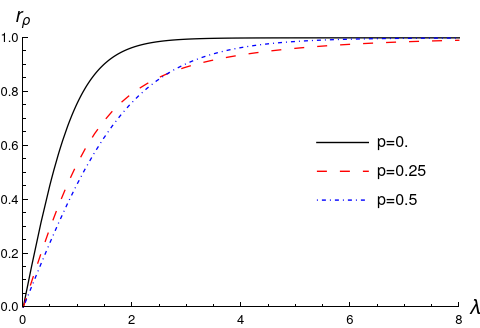
\includegraphics[width=0.6\linewidth]{chapter2/figures/r(lambda).png}
    \caption{$r_{\rho_{\ef}}$ como función de $\lambda$ para diferentes valores de $p_{1}$ en el caso en que $n=2$.}
    \label{fig:r(lambda)}
\end{figure}
Cada multiplicador de Lagrange queda determinado de forma única a través de cantidades experimentales según 
\begin{equation}
    \lambda_{i}=\rfroml^{-1}(r_{\rho_{\ef}}) \frac{\expval{\pauli{i}}}{r_{\rho_{\ef}}},
\end{equation}
y, por supuesto,
\begin{equation}
    \lambda=\rfroml^{-1}(r_{\rho_{\ef}})\nonumber
\end{equation}
Aunque siempre exista, no es posible hallar una expresión de $\rfroml^{-1}$ para cualquier valor de $p$ debido a que la ecuación (\ref{eq:r(lambda)}) es una ecuación trascendental. Por esto, para escribir al estado de máxima entropía como una función de cantidades medibles, nos tendremos que conformar con llamar a $\rfroml^{-1}$ de manera explícita.

\subsection{Otra expresión del estado de máxima entropía}

\acnote{Revisar si la rama principal es justificación suficiente para agarrar la potencia}

\acnote{Revisado, como las matrices son semidefinidas positivas, su logaritmo es único.}

La ecuación (\ref{eq:MaxEntSeparable}) sugiere que el estado de máxima entropía puede expresarse como producto tensorial de potencias de un mismo estado. En efecto, dado un real $q$ y una matriz cuadrada $A$, la potenciación $A^{q}$ puede escribirse como $e^{q \ln A}$. Como las matrices $e^{\sum_{i}\lambda_{i}\pauli{i}}$ son semidefinidas positivas, su logaritmo es único. Entonces,
\begin{equation}
    \varrho_{\max}=\Motimes_{j=1}^{n}\frac{1}{Z_{j}}e^{p_{j}\sum_{k}\lambda_{k}\pauli{k}}=\Motimes_{j=1}^{n}\frac{1}{Z_{j}}\qty(e^{\sum_{k}\lambda_{k}\pauli{k}})^{p_{j}}.\nonumber
\end{equation}
En virtud de (\ref*{ap:PauliRealExp}), se cumple que
\begin{align}
  \varrho_{\max}=&\Motimes_{j=1}^{n}\frac{\qty(\cosh{\lambda}(\Id+\tanh{\lambda}(\paulivec{r_{\rho}})))^{p_{j}}}{\Tr[\qty(\cosh{\lambda}(\Id+\tanh{\lambda}(\paulivec{r_{\rho}})))^{p_{j}}]}\nonumber\\
  =&\Motimes_{j=1}^{n}\frac{\qty(\Id+\tanh{\lambda}(\paulivec{r_{\rho}}))^{p_{j}}}{\Tr[\qty(\Id+\tanh{\lambda}(\paulivec{r_{\rho}}))^{p_{j}}]}.\nonumber
\end{align}
Definimos
\begin{equation}\label{eq:Xi}
  \Xi_{\max}=\frac{1}{2}(\Id+\tanh{\lambda}(\paulivec{r_{\rho}})).
\end{equation}
de tal manera que 
\begin{equation}\label{eq:MaxEntSeparablePower}
  \varrho_{\max}=\Motimes_{j=1}^{n}\frac{(\Xi_{\max})^{p_{j}}}{\Tr[ (\Xi_{\max})^{p_{j}}]}
\end{equation}

\subsection{La asignación de máxima entropía}

El estado de máxima entropía nos otorga una herramienta de asignación para los estados accesibles. Después de todo, requerimos de una asignación razonable que pueda ser propagada según la dinámica microscópica conocida. Sea $\rho_{\ef}\in\densityspace{2}$ un estado efectivo, entonces definimos a la aplicación de asignación de máxima entropía como

\begin{gather}\label{eq:MaxEntAss}
    \mcA_{\mcC}^{\max}:\densityspace{2}\rightarrow\densityspace{2^{n}}\nonumber\\
    \rho_{\ef} \mapsto \Motimes_{j=1}^{n}\frac{1}{Z_{j}}\text{exp}\qty(p_{j}\sum_{k=1}^{3}\lambda_{k}\sigma_{k}).
\end{gather}
donde la dependencia de la asignación en el modelo de grano grueso se indica mediante un subíndice. Nótese que según los valores que puedan tomar las diferentes probabilidades, el \textit{estado asignado} tendrá diferentes propiedades. En dos casos particulares, la aplicación de asignación es lineal: cuando $p_{1}=1$ y cuando $p_{j}=\frac{1}{n}\forall j$.

Si $p_{1}=1$ entonces se eliminan los términos de error, y el estado de máxima entropía es simplemente
\begin{equation}
    \varrho_{\max}=\rho_{\ef}\otimes\Id^{2^{n-1}}.\nonumber
\end{equation}
Si, por otro lado, $p_{j}=\frac{1}{n}\forall j$, entonces el estado de máxima entropía es
\begin{equation}
    \varrho_{\max}=\qty[\frac{1}{Z}\text{exp}\qty(\frac{1}{n}\sum_{k=1}^{3}\lambda_{k}\sigma_{k})]^{\otimes n}=(\rho')^{\otimes n}.\nonumber
\end{equation}
Si se pasa este estado por la aplicación de grano grueso correspondiente el resultado es 
\begin{equation}
    \mcC[\varrho_{\max}]=\sum_{j=1}^{n}\frac{1}{n}\rho'=\rho',\nonumber
\end{equation}
de  lo que se concluye que
\begin{equation*}
    \rho'=\rho_{\ef},
\end{equation*}
y que por lo tanto el estado asignado es simplemente
\begin{equation}
    \mcA_{\mcC}^{\max}(\rho_{\ef})=\rho_{\ef}^{\otimes n}.\nonumber
\end{equation}
El caso $p_{1}=1$ debe verse como un caso límite: aquel en el que la medición no es borrosa. Este trabajo estudiará el límite $p_{1}\rightarrow 1$ como el escenario en el que la probabilidad de detectar la partícula equivocada es pequeña. Por otro lado, si $p_{j}=\frac{1}{n}\forall j$, la asignación de máxima entropía resulta en $n$ partículas idénticas.